% Created 2016-04-12 Tue 01:13
\documentclass[9pt,b5paper]{article}
\usepackage{graphicx}
\usepackage{xcolor}
\usepackage{xeCJK}
\setCJKmainfont{SimSun}
\usepackage{longtable}
\usepackage{float}
\usepackage{textcomp}
\usepackage{geometry}
\geometry{left=0cm,right=0cm,top=0cm,bottom=0cm}
\usepackage{multirow}
\usepackage{multicol}
\usepackage{listings}
\usepackage{algorithm}
\usepackage{algorithmic}
\usepackage{latexsym}
\usepackage{natbib}
\usepackage{fancyhdr}
\usepackage[xetex,colorlinks=true,CJKbookmarks=true,linkcolor=blue,urlcolor=blue,menucolor=blue]{hyperref}


\lstset{language=c++,numbers=left,numberstyle=\tiny,basicstyle=\ttfamily\small,tabsize=4,frame=none,escapeinside=``,extendedchars=false,keywordstyle=\color{blue!70},commentstyle=\color{red!55!green!55!blue!55!},rulesepcolor=\color{red!20!green!20!blue!20!}}
\author{deepwaterooo}
\date{\today}
\title{Tetris - Basic Implementation Practice for Android}
\hypersetup{
  pdfkeywords={},
  pdfsubject={},
  pdfcreator={Emacs 24.3.1 (Org mode 8.2.7c)}}
\begin{document}

\maketitle
\tableofcontents


\section{Better version, pretty good}
\label{sec-1}
\begin{itemize}
\item OpenGL 3D version status: 
\begin{itemize}
\item Basic game flow debugging. just fixed one bug today.
\item Will read and work on the existing code, make the app run without crashing down (need add a few buttons for first page, \& I had that already), and try to get an initial 3d frames and a couple of blocks showing out.
\item Will try to finish the \textbf{Undertable} repository today.
\item Will work on this project during the day, go to class in the evening, and report status later in late evening.
\item 
\item Still trying to adapt from the TetrisGlar app, and worked on the codes that are necessary for a real 3D instead of pseudo-3d.
\item Understand the math part better, to remove unnessary background parts, mirror parts, beside making 2d ==> 3d, rotation could be modified to be better.
\item Will continue work on this one today after updated "\textbf{Undertable Blackmail}" repository.
\item This project is still on and updating, please don't think I could give up this one. Even I made limited progress someday, but I will make this project work after working on it day by day.
\item 
\item I believe about MVP, I am correct now, and I am using the same world center now.
\item For translation, rotation, calculation transformation matrix, I still have to write these utilities in order for my Cubes/Blocks to move.
\item And I should NOT have been blocked by this drawing for so long, but at least now I know I am correct.
\item Will work on Cube==>Block==>Model game flow on Monday, and will update on Monday latest in the evening.
\item 
\item Move shader and drawing back to Cube, my flow of drawing direction is inverted. I could write and get my own UNV R$^{\text{T}}$ matrix and translation matrix (though it's just a wrapper from OpengGL api functions) by calculating from setLookAtM function parameters, I believe this matrix should NOT multiply on my translated \& scaled coordinates.
\item (model translate ==> model rotate ==> V * ModelTransRotate result ==> P * V * M, left multiply for opengl matrix, which is WRONG). the correct should be:
\item Vector(ofNewVertex) = M$_{\text{Projection[from}}$ screen ratio] * (M$_{\text{Translation[opposite}}$ eye position] * (M$_{\text{Rotation[inverse}}$ UNV directions, from LookAt parameters for Q$^{\text{(-1)}}$ = Q$^{\text{T]}}$ * Vector(ofOriginalVertex))), now is right
\item Block center should be an important concept here, and I need to add the 3 parameters back, because they need to rotate and translate, scale later on depends on the Block center.
\item 
\item Have spent two days tried to review someone else's code, but it was too complicated rather than developping my own code ( tetrisglar$_{\text{d9qpjwxc}}$.apk is included in home directory for referrencing).
\item So from late this afternoon, working on my own codes, partially still referring to the other apk, but it's my flow-chart-ideas and implementation now.
\item I believe I got at least some ideas for most of the basic ideas and OpenGL technical difficulties, so the implementation won't be too hard.
\item game layout structure:
\end{itemize}
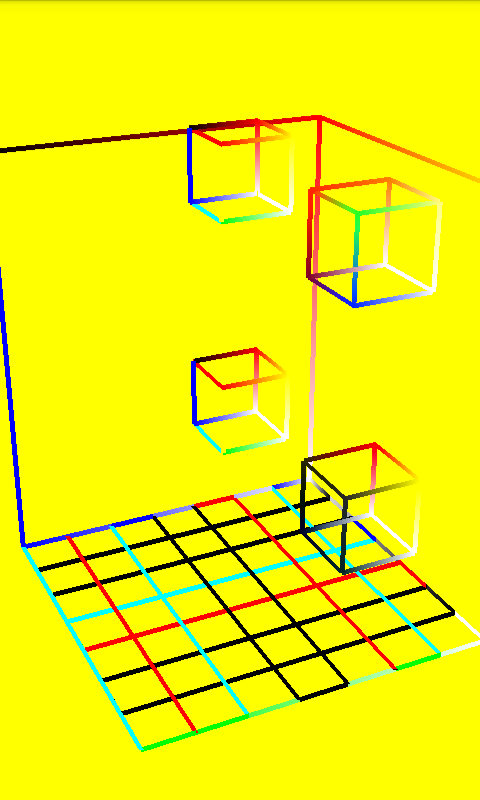
\includegraphics[width=.9\linewidth]{./Screenshot_2016-04-07-11-58-28.png}
\item most challenge part for tonight, matrix translations \& rotations\ldots{}.will continue work on it tonight

\item a video for this Tetris game can be directly watched at \url{https://www.youtube.com/watch?v=Ht4NOrEUtFk}
\item A video for the previous DrawingFun Android App can be watched at \url{https://www.youtube.com/watch?v=YV78Tk5--5M} , or by searching \textbf{deepwaterooo Wang}.
\item 
\item Starting my trial for OpenGL ES, need to figure out how to draw a game board.
\item Won't be able to work on it this weekend, but will work on it later on.
\item 
\item These video will serve as the indication that as an educated well practiced graduated student, I have the solid technological background, my problem solving skills, the spirit of implementing whatever ideas for apps that I feel I am capable, as well as confidence as an entry level mobile app programmer.
\item For the Tetris game, it's NOT the best product in my mind yet (though it is pretty good now and I will make it a my version of Tetris), but I want to record it so that more friends can enjoy the so far already achieved progress, and for those who just know me would be able to know what is my interested field.
\item By using SurfaceView who has a separate thread for drawing/painting, this game actually it pretty good already, at least should be about 80 out of 100.
\item Though I will continuous refine this game later on when I have time (Better version will be recorded and uploaded later within a month or so.), but I won't be able to work on it day in and day out recently, having other things occupied.
\end{itemize}

\section{References}
\label{sec-2}
\subsection{3D design}
\label{sec-2-1}
\begin{itemize}
\item c++ version: \url{https://github.com/matachi/tetris-cpp}
\item refer 6 \url{http://www.oschina.net/question/614942_62370}
\item \url{http://www.oschina.net/question/565065_67280}
\item triangle: \url{http://stackoverflow.com/questions/9945321/triangle-opengl-in-android}
\item \url{https://gist.github.com/SebastianJay/3316001}
\item 射线拾取: \url{http://itdocument.com/479827008/}
\item 旋转及手势: \url{http://vaero.blog.51cto.com/4350852/790620}
\item 2 \url{http://vaero.blog.51cto.com/4350852/790637}
\item \url{http://www.lai18.com/content/951343.html}
\item opengl选择与反馈: \url{http://zhidao.baidu.com/question/496046750245095004.html}
\item \url{http://wenku.baidu.com/view/58190d1efad6195f312ba6f7.html}
\item c++ \url{http://blog.csdn.net/u010223072/article/details/45369075}
\item \url{http://codercdy.com/2015/06/17/openglxue-xi-bi-ji-xuan-ze-he-fan-kui/}
\item \url{https://books.google.com/books?id=u6EHM_OzaFQC&pg=PA1987&lpg=PA1987&dq=opengl\%E9\%80\%89\%E6\%8B\%A9\%E4\%B8\%8E\%E5\%8F\%8D\%E9\%A6\%88&source=bl&ots=L9Y66QSEhu&sig=f1h_RadXRDFsa9L5IY430HGTG34&hl=en&sa=X&ved=0ahUKEwjA6vTRo_jLAhVH3mMKHQIXBxYQ6AEIPDAE#v=onepage&q=opengl\%E9\%80\%89\%E6\%8B\%A9\%E4\%B8\%8E\%E5\%8F\%8D\%E9\%A6\%88&f=false}
\item c++ codes: \url{http://dev.gameres.com/program/Visual/3D/Selection.htm}
\item 画线: c++ \url{http://www.programgo.com/article/43724048060/}
\item draw line: \url{http://www.linuxidc.com/Linux/2011-09/42307p3.htm}
\item \url{http://stackoverflow.com/questions/9217702/open-gl-es-2-0-drawing-a-simple-line}
\item 距阵变换: \url{http://www.cnblogs.com/caster99/p/4780984.html}
\item \url{http://www.flakor.cn/2014-05-15-384.html}
\item shader util: \url{http://blog.csdn.net/shulianghan/article/details/17020359}
\item 详解距阵变换:\url{http://www.cnblogs.com/kesalin/archive/2012/12/06/3D_math.html}
\item \url{http://mail.cfanz.cn/index.php?c=article&a=read&id=270244}
\item one example: \url{http://www.apkbus.com/blog-99192-39498.html}
\item ex2 for shader matrix: \url{http://www.voidcn.com/blog/peanut__love/article/p-2891341.html}
\item 西蒙iPhone-OpenGL ES 中文教程专题: \url{http://www.cocoachina.com/special/2010/0126/404.html}
\item 运动: \url{http://www.cocoachina.com/bbs/read.php?tid-7601-fpage-10.html}
\item 
\item 距阵: \url{http://blog.csdn.net/wangdingqiaoit/article/details/39010077}
\item \url{http://blog.csdn.net/popy007/article/details/5120158} UNV
\item \url{http://www.tqcto.com/article/mobile/23873.html} eye
\item \url{http://blog.csdn.net/wangdingqiaoit/article/details/39937019}
\item 
\item 
\item \url{https://developer.apple.com/library/ios/documentation/3DDrawing/Conceptual/OpenGLES_ProgrammingGuide/Introduction/Introduction.html}
\item 
\item 
\item 
\item 
\item 
\item 
\item 
\end{itemize}

\subsection{GLSurfaceView}
\label{sec-2-2}
\begin{itemize}
\item opengl: \url{http://androidblog.reindustries.com/a-real-open-gl-es-2-0-2d-tutorial-part-1/}
\item Graphics architecture: \url{https://source.android.com/devices/graphics/architecture.html}
\item \url{http://stackoverflow.com/questions/5169338/android-deciding-between-surfaceview-and-opengl-glsurfaceview}
\item \textbf{引路蜂} better: \url{http://blog.csdn.net/mapdigit/article/details/7526556}
\item 真正的3D图形: \url{http://www.imobilebbs.com/wordpress/archives/1554}
\item a Cube: \url{http://www.oschina.net/question/4873_28325}
\item modification: \url{https://github.com/googleglass/gdk-apidemo-sample/blob/master/app/src/main/java/com/google/android/glass/sample/apidemo/opengl/Cube.java}
\item Android OpenGL ES 简明开发教程小结: \url{http://www.imobilebbs.com/wordpress/archives/1583}
\item 
\item 
\item 

\item \url{http://hellosure.github.io/android/2015/06/01/android-glsurfaceview/}
\item \url{http://ju.outofmemory.cn/entry/172850}
\item 画图: \url{http://www.mobile-open.com/2015/81568.html}
\item \url{http://tangzm.com/blog/?p=20}
\item \url{http://www.apkbus.com/blog-99192-39584.html}
\item onDrawFrame intro: \url{http://www.jayway.com/2009/12/03/opengl-es-tutorial-for-android-part-i/}
\item failed: \url{http://stackoverflow.com/questions/28711850/android-opengl-how-to-draw-a-rectangle}
\item onTouchEvent: \url{http://blog.csdn.net/niu_gao/article/details/8673662}
\item volatile \url{http://www.voidcn.com/blog/fanfanxiaozu/article/p-3668133.html}
\item \url{http://mobile.51cto.com/aengine-437172.htm}
\item OpenGLES related: \url{http://stackoverflow.com/questions/9945321/triangle-opengl-in-android}
\item OpenGL ES 2.0 Sample Code: \url{http://androidbook.com/item/4254}
\item intros:详解 \url{http://blog.csdn.net/niu_gao/article/details/7566297}
\item 画线: \url{http://www.cnblogs.com/lhxin/archive/2012/06/01/2530828.html}
\item \url{http://bbs.9ria.com/thread-201740-1-1.html}
\item \url{http://imgtec.eetrend.com/blog/5078}
\item draw a ball \url{http://shikezhi.com/html/2015/android_1022/561912.html}
\item for Board c++: \url{http://www.jiancool.com/article/24471349949/}
\item possible? \url{http://code1.okbase.net/codefile/CCFormatter.java_2015072733469_393.htm}
\item \url{http://www.mobile-open.com/2015/80379.html}
\end{itemize}

\subsection{eventQueue vs SurfaceView threads}
\label{sec-2-3}
\begin{itemize}
\item Deeper summary, android graphics architecture: \url{http://hukai.me/android-deeper-graphics-architecture/}
\item 2 threads, load, read, \url{http://blog.csdn.net/hellogv/article/details/5986835}
\end{itemize}
\subsection{Canvas Path subclass}
\label{sec-2-4}
\begin{itemize}
\item how to define drawLine to be drawShapes?
\end{itemize}
\subsection{SurfaceView}
\label{sec-2-5}
\begin{itemize}
\item Surface runnable \url{http://android.okhelp.cz/surfaceview-implements-runnable-android-code/}
\item Example: \url{http://technicalsearch.iteye.com/blog/1967616}
\item \url{http://www.jcodecraeer.com/a/anzhuokaifa/androidkaifa/2012/1201/656.html}
\item Event Queue: \url{http://www.leestorm.com/post/17.html}
\item lockCanvas(Rect小区) \url{http://blog.csdn.net/alexander_xfl/article/details/13000347}
\item example: \url{http://fanli7.net/a/JAVAbiancheng/ANT/20120424/160203.html}
\item MotionEvent: \url{http://android.jobbole.com/82072/}
\item surfaceview双缓冲: \url{http://blog.csdn.net/cnbloger/article/details/7404485}
\item sth worth try: \url{http://www.lxway.com/969295592.htm}
\item Dont Understand: \url{http://blog.sina.com.cn/s/blog_5a6f39cf01012rtv.html}
\item tried: \url{http://bbs.csdn.net/topics/370074255} drawBitmap 2 canvas
\item slightly complicated: \url{http://www.lxway.com/148606691.htm}
\item slightly complicated: \url{http://www.lxway.com/186948856.htm}
\end{itemize}

\subsection{gestures}
\label{sec-2-6}
\begin{itemize}
\item \url{http://www.cnblogs.com/akira90/archive/2013/03/10/2952886.html}
\item Android 触摸手势基础 官方文档概览: \url{http://www.lxway.com/445554926.htm}
\item 手势: \url{http://wiki.jikexueyuan.com/project/material-design/patterns/gestures.html}
\item \url{http://www.lxway.com/601620614.htm}
\item \url{http://www.lxway.com/282219004.htm}
\item \url{http://www.lxway.com/906451412.htm}
\item \url{http://www.lxway.com/146619692.htm}
\item \url{http://www.lxway.com/4420294641.htm}
\item \url{http://www.lxway.com/155059816.htm}
\item \url{http://www.lxway.com/4019928952.htm}
\item 例子: \url{http://bbs.chinaunix.net/thread-3634477-1-1.html}
\item 例子: \url{http://www.bestappsmarket.com/p/app?appId=1192877&title=tetris-\%E4\%BF\%84\%E7\%BD\%97\%E6\%96\%AF\%E6\%96\%B9\%E5\%9D\%97}
\item 例子: \url{http://bbs.chinaunix.net/thread-3634477-1-1.html}

\item iTetris: \url{http://searchapp.soft4fun.net/article/information/iTetris\%20\%E4\%BF\%84\%E7\%BD\%97\%E6\%96\%AF\%E6\%96\%B9\%E5\%9D\%97/313319}
\item left right: \url{http://www.jb51.net/article/77028.htm}
\item AI: \url{http://www.cnblogs.com/youngshall/archive/2009/03/24/1420682.html}
\item 
\item 3/11/2016 Friday
\item \url{https://github.com/Almeros/android-gesture-detectors} mac
\item \url{http://www.jcodecraeer.com/a/anzhuokaifa/androidkaifa/2015/0211/2467.html}
\item \url{http://www.hejun.biz/81.html}
\item \url{http://www.jb51.net/article/38166.htm}
\item \url{http://www.jb51.net/article/37717.htm}
\item \url{http://mobile.51cto.com/aprogram-394841.htm}

\item TetrisBattle特殊轉入教學(Z S J L I)
\begin{itemize}
\item \url{https://www.youtube.com/watch?v=zW6Gp_7jl9I}
\end{itemize}
\item 推箱子: 第11章 Android游戏开发视频教程 益智游戏——推箱子
\begin{itemize}
\item \url{https://www.youtube.com/watch?v=glzxII1-P0A} 2.5D
\end{itemize}
\item 祖码游戏的设计与实现
\end{itemize}
% Emacs 24.3.1 (Org mode 8.2.7c)
\end{document}